% This LaTeX was auto-generated from MATLAB code.
% To make changes, update the MATLAB code and export to LaTeX again.

\documentclass{article}

\usepackage[utf8]{inputenc}
\usepackage[T1]{fontenc}
\usepackage{lmodern}
\usepackage{graphicx}
\usepackage{color}
\usepackage{hyperref}
\usepackage{amsmath}
\usepackage{amsfonts}
\usepackage{epstopdf}
\usepackage[table]{xcolor}
\usepackage{matlab}

\sloppy
\epstopdfsetup{outdir=./}
\graphicspath{ {./Lab02_images/} }

\begin{document}

\matlabtitle{LAB 2: FREQUENCY DOMAIN AND TRANSFER FUNCTIONS}

\begin{matlabcode}
%---------------------------------------
% Fill in your student Name and ID.
Students.Name = 'Seyed Yazdan Zinati';
Students.ID = '260928077';
%---------------------------------------
\end{matlabcode}


\matlabheading{\textbf{0. Objectives}}

\begin{par}
\begin{flushleft}
The purpose of this lab is to overview the basic \texttt{\textbf{MATLAB}} functions in linear systems and control. At the end of this lab, you will be able to plot the step and impulse response of a rational transfer function and analyze with first and second order transfer functions.
\end{flushleft}
\end{par}

\matlabheading{\textbf{1. Introduction}}

\begin{par}
\begin{flushleft}
The first step in the design of a control system is to identify a mathematical model of the system. Such a mathematical model could be derived either from physical laws or from experimental data. For Linear Time Invariant (LTI) systems, we only need to identify the impulse response or it's frequency-domain representation: the transfer function.
\end{flushleft}
\end{par}

\begin{par}
\begin{flushleft}
In this lab, we introduce how to model transfer functions in \texttt{\textbf{MATLAB}}. There are various methods to define a transfer function in \texttt{\textbf{MATLAB}}. As an example, suppose we have a system described by the following constant coefficient linear differential equation:
\end{flushleft}
\end{par}

\begin{par}
$$a_2 {{\frac{d^2 y(t)}{dt}+a_1 {{\frac{dy(t)}{dt}+a_0 y(t)=b_1 {{\frac{du(t)}{dt}+b_0 u(t)}}}}}}$$
\end{par}

\begin{par}
\begin{flushleft}
We know that the transfer function of this system is
\end{flushleft}
\end{par}

\begin{par}
$$H(s)={{\frac{Y(s)}{U(s)}={{\frac{b_1 s+b_0 }{a_2 s^2 +a_1 s+a_0 }}}}}$$
\end{par}

\begin{par}
\begin{flushleft}
Suppose $a_0 =2$, $a_1 =3$, $a_2 =1$, $a_3 =1$, $b_0 =2$, $b_1 =2$.
\end{flushleft}
\end{par}

\begin{par}
\begin{flushleft}
The first method of specifying the function is to literally type out this expression. We first define the symbol $s$ using the \texttt{\textbf{tf}} function and then define the transfer function $H$ in terms of $s$. For example:
\end{flushleft}
\end{par}

\begin{matlabcode}
% Assign values to the coefficients
a2 = 1;
a1 = 3;
a0 = 2;
b1 = 2;
b0 = 6;
% Define s symbolically in frequency domain
s = tf('s');
\end{matlabcode}


\begin{par}
\begin{flushleft}
Then we can directly define the transfer function as follows.
\end{flushleft}
\end{par}

\begin{matlabcode}
H1 = (b1 * s + b0) / (a2 * s^2 + a1 * s + a0)
\end{matlabcode}
\begin{matlaboutput}
H1 =
 
     2 s + 6
  -------------
  s^2 + 3 s + 2
 
Continuous-time transfer function.
\end{matlaboutput}


\begin{par}
\begin{flushleft}
The second method is to directly specify the polynomials of the numerator and the denominators.
\end{flushleft}
\end{par}

\begin{matlabcode}
% Define the numerator
num = [b1, b0];
% Define the denominator
den = [a2, a1, a0];
% Define the transfer function
H2 = tf(num, den)
\end{matlabcode}
\begin{matlaboutput}
H2 =
 
     2 s + 6
  -------------
  s^2 + 3 s + 2
 
Continuous-time transfer function.
\end{matlaboutput}


\begin{par}
\begin{flushleft}
Another way to define the transfer function is to use the gain, poles and zeros. Let's reconsider the above transfer function in pole-zero form.
\end{flushleft}
\end{par}

\begin{par}
$$H(s)=2{{\frac{s+2}{(s+1)(s+2)}}}$$
\end{par}

\begin{par}
\begin{flushleft}
We can specify the transfer function in the pole zero form using the following code.
\end{flushleft}
\end{par}

\begin{matlabcode}
k = 2; % The gain
z = [-3]; % The set of zeros
p = [-1, -2]; % The set of poles
H3 = zpk(z, p, k) % Define the transfer function
\end{matlabcode}
\begin{matlaboutput}
H3 =
 
    2 (s+3)
  -----------
  (s+1) (s+2)
 
Continuous-time zero/pole/gain model.
\end{matlaboutput}


\begin{par}
\begin{flushleft}
There are other forms of using the \texttt{\textbf{zpk}} function. Use \texttt{\textbf{doc zpk}} for more information.
\end{flushleft}
\end{par}

\begin{par}
\begin{flushleft}
It is possible to identify the poles and zeros of a \textbf{rational} transfer function using \texttt{\textbf{tf2zp}}:
\end{flushleft}
\end{par}

\begin{matlabcode}
[z, p, k] = tf2zp(num, den)
\end{matlabcode}
\begin{matlaboutput}
z = -3
p = 2x1    
    -2
    -1

k = 2
\end{matlaboutput}


\matlabheading{\textbf{2. Plotting Impulse and Step Responses}}

\begin{par}
\begin{flushleft}
To plot the impulse response of a transfer function, one can use \texttt{\textbf{impulse(sys)}}. To plot the step response, one can use \texttt{\textbf{step(sys)}}. As an example, we plot the impulse and step responses of the system defined in the previous section:
\end{flushleft}
\end{par}

\begin{matlabcode}
T = 10; % Final time value
figure;
impulse(H1, T)
\end{matlabcode}
\begin{center}
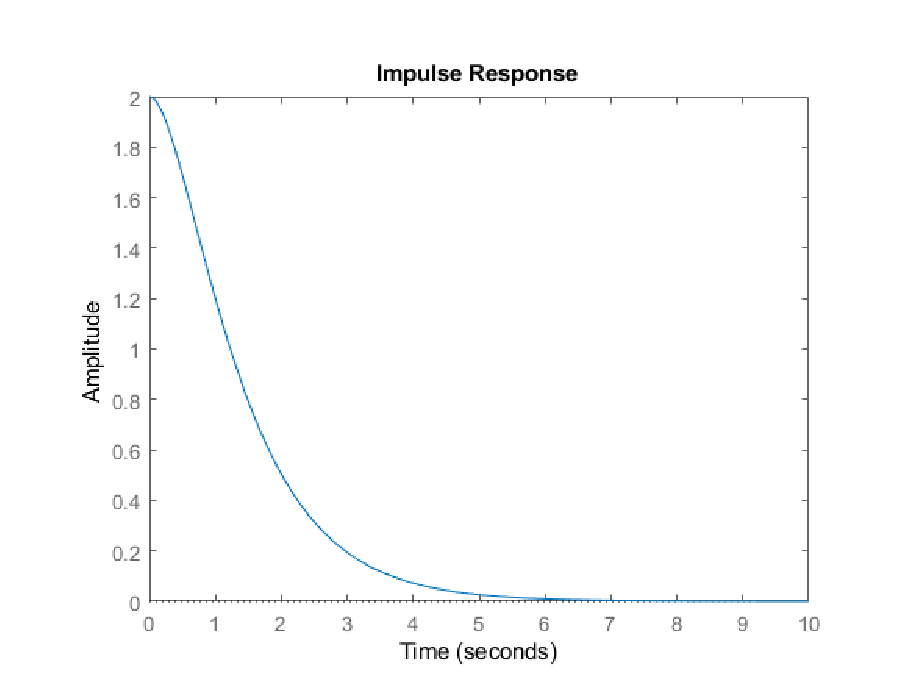
\includegraphics[width=\maxwidth{56.196688409433015em}]{figure_0.eps}
\end{center}


\begin{matlabcode}
figure;
step(H1, T)
\end{matlabcode}
\begin{center}
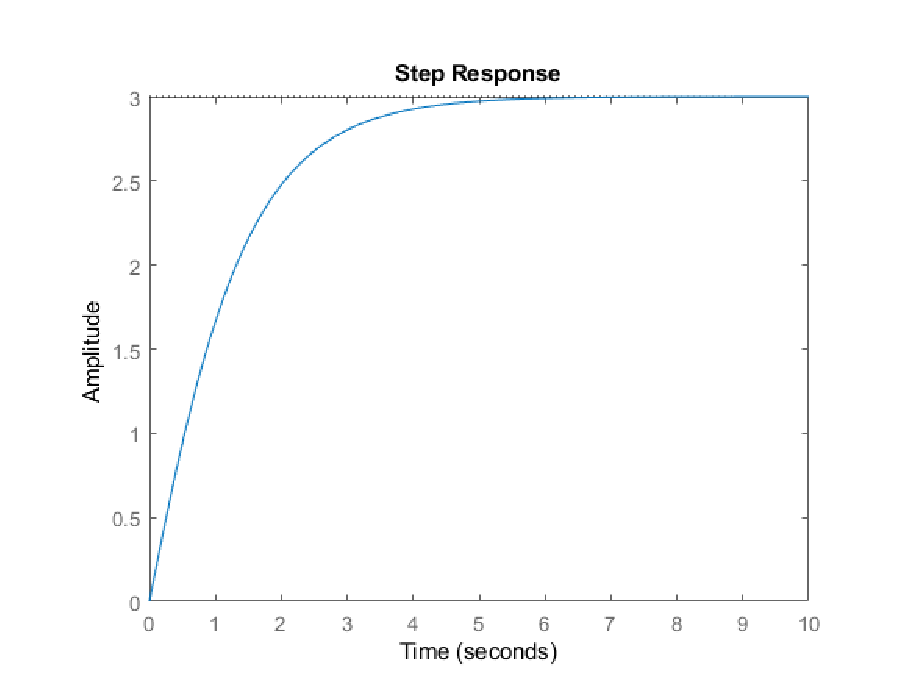
\includegraphics[width=\maxwidth{56.196688409433015em}]{figure_1.eps}
\end{center}


\begin{par}
\begin{flushleft}
To find the poles and zeros of a transfer function, use \texttt{\textbf{pole(system)}} and \texttt{\textbf{zero(systems)}}. To plot the pole-zero plot, use \texttt{\textbf{pzplot(system)}}. For example, for the system defined above, the poles are
\end{flushleft}
\end{par}

\begin{matlabcode}
pole(H1)
\end{matlabcode}
\begin{matlaboutput}
ans = 2x1    
    -2
    -1

\end{matlaboutput}


\begin{par}
\begin{flushleft}
and the zeros are
\end{flushleft}
\end{par}

\begin{matlabcode}
zero(H1)
\end{matlabcode}
\begin{matlaboutput}
ans = -3
\end{matlaboutput}


\begin{par}
\begin{flushleft}
We can show the pole-zero plot using
\end{flushleft}
\end{par}

\begin{matlabcode}
pzplot(H1)
\end{matlabcode}
\begin{center}
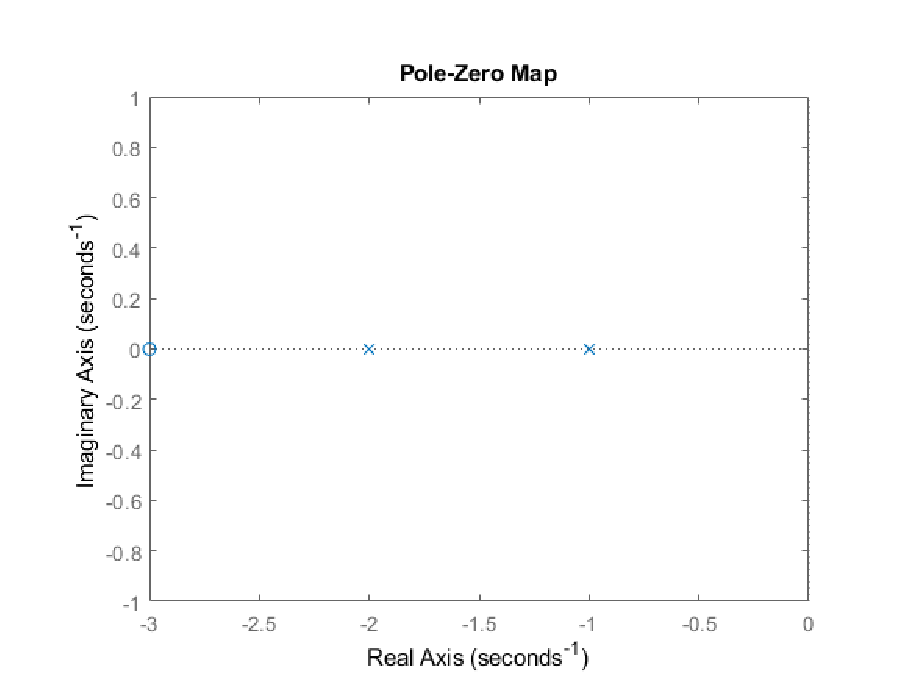
\includegraphics[width=\maxwidth{56.196688409433015em}]{figure_2.eps}
\end{center}


\matlabheading{\textbf{Interconnecting systems}}

\begin{par}
\begin{flushleft}
To get the transfer function for two systems connected in feedback, use
\end{flushleft}
\end{par}

\begin{matlabcode}
H = feedback(H1, H2) % Feedback or closed-loop interconnection of systems
\end{matlabcode}
\begin{matlaboutput}
H =
 
     2 s^3 + 12 s^2 + 22 s + 12
  --------------------------------
  s^4 + 6 s^3 + 17 s^2 + 36 s + 40
 
Continuous-time transfer function.
\end{matlaboutput}


\begin{par}
\begin{flushleft}
Use \texttt{\textbf{doc feedback}} for more information.
\end{flushleft}
\end{par}

\matlabheading{\textbf{3. System Response characteristics}}

\begin{par}
\begin{flushleft}
Consider the following step response of an unknown transfer function.
\end{flushleft}
\end{par}

\begin{par}
\begin{flushleft}
\textless{}\textless{}fig\_lab02\_secondorder.png\textgreater{}\textgreater{}
\end{flushleft}
\end{par}

\begin{par}
\begin{flushleft}
Depending on the location of the zeros and poles in a transfer function, it is possible to define a system response by the following characteristics:
\end{flushleft}
\end{par}

\begin{itemize}
\setlength{\itemsep}{-1ex}
   \item{\begin{flushleft} Rise time ($t_r$): is the time it takes the system to reach to rise from 10\% to 90\% of its final value. \end{flushleft}}
   \item{\begin{flushleft} Peak time ($t_p$): is the time until the response hits its maximum overshoot. \end{flushleft}}
   \item{\begin{flushleft} Overshoot ($M_p$): is the peak value of the step response of the system. \end{flushleft}}
   \item{\begin{flushleft} Settling time ($t_s$): is the time for the response to settle within $\pm \Delta$ \% of its final value. \end{flushleft}}
\end{itemize}

\begin{par}
\begin{flushleft}
It is possible to find these values in \texttt{\textbf{MATLAB}} given a transfer function. \texttt{\textbf{stepinfo(sys)}} computes the step-response characteristics for a dynamic system model. For example
\end{flushleft}
\end{par}

\begin{matlabcode}
stepinfo(H1)
\end{matlabcode}
\begin{matlaboutput}
ans = 
        RiseTime: 2.4200
    SettlingTime: 4.1960
     SettlingMin: 2.7023
     SettlingMax: 2.9974
       Overshoot: 0
      Undershoot: 0
            Peak: 2.9974
        PeakTime: 7.3222

\end{matlaboutput}


\matlabheading{\textit{Question 1 (2 marks)}}

\begin{par}
\begin{flushleft}
For $\xi =\lbrace 0.25,0.75,1,2\rbrace$, plot the step response \textbf{(for 25 sec)} and identify the characteristics of the transient response of the following system
\end{flushleft}
\end{par}

\begin{par}
$$G(s)={{\frac{1}{s^2 +2\xi s+1}}}$$
\end{par}

\begin{matlabcode}
%------------------------------------
% defining the transfer function 

xi = 0.25;  

% define numerator and denominator
num = 1;
den = [1, 2*xi, 1];
G1 = tf(num, den)
\end{matlabcode}
\begin{matlaboutput}
G1 =
 
         1
  ---------------
  s^2 + 0.5 s + 1
 
Continuous-time transfer function.
\end{matlaboutput}
\begin{matlabcode}

%------------------------------------
% plotting the step response

T = 25; % final time value

figure;
step(G1, T)
\end{matlabcode}
\begin{center}
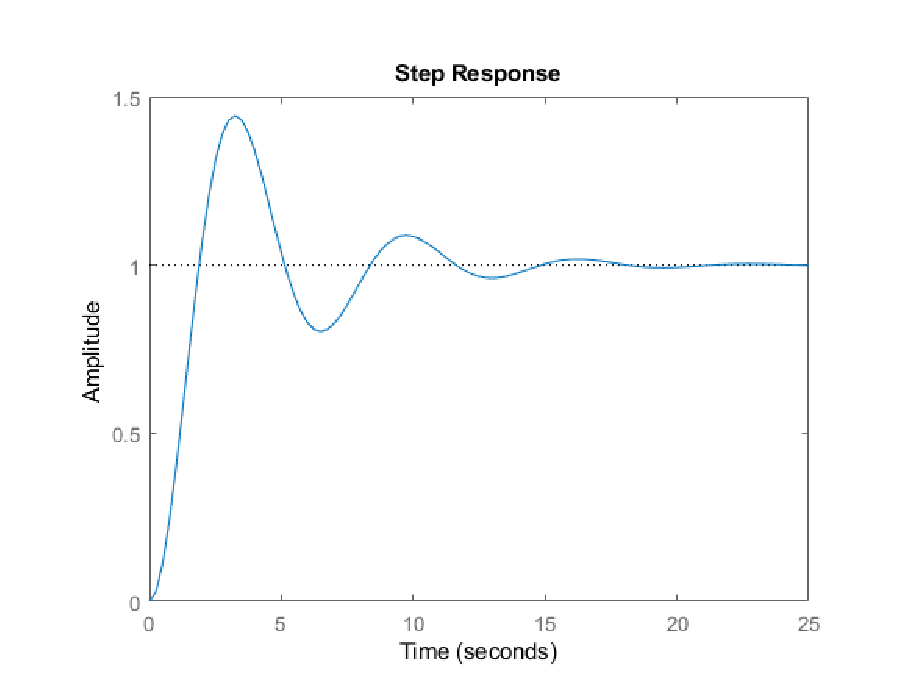
\includegraphics[width=\maxwidth{56.196688409433015em}]{figure_3.eps}
\end{center}
\begin{matlabcode}

%------------------------------------
% identifying the characteristics 
% of the transient response
stepinfo(G1)
\end{matlabcode}
\begin{matlaboutput}
ans = 
        RiseTime: 1.2687
    SettlingTime: 14.1159
     SettlingMin: 0.8027
     SettlingMax: 1.4432
       Overshoot: 44.3235
      Undershoot: 0
            Peak: 1.4432
        PeakTime: 3.3157

\end{matlaboutput}


\begin{matlabcode}
%------------------------------------
% defining the transfer function 

xi = 0.75;

% define numerator and denominator
num = 1;
den = [1, 2*xi, 1];
G2 = tf(num, den)
\end{matlabcode}
\begin{matlaboutput}
G2 =
 
         1
  ---------------
  s^2 + 1.5 s + 1
 
Continuous-time transfer function.
\end{matlaboutput}
\begin{matlabcode}

%------------------------------------
% plotting the step response

T = 25; % final time value

figure;
step(G2, T)
\end{matlabcode}
\begin{center}
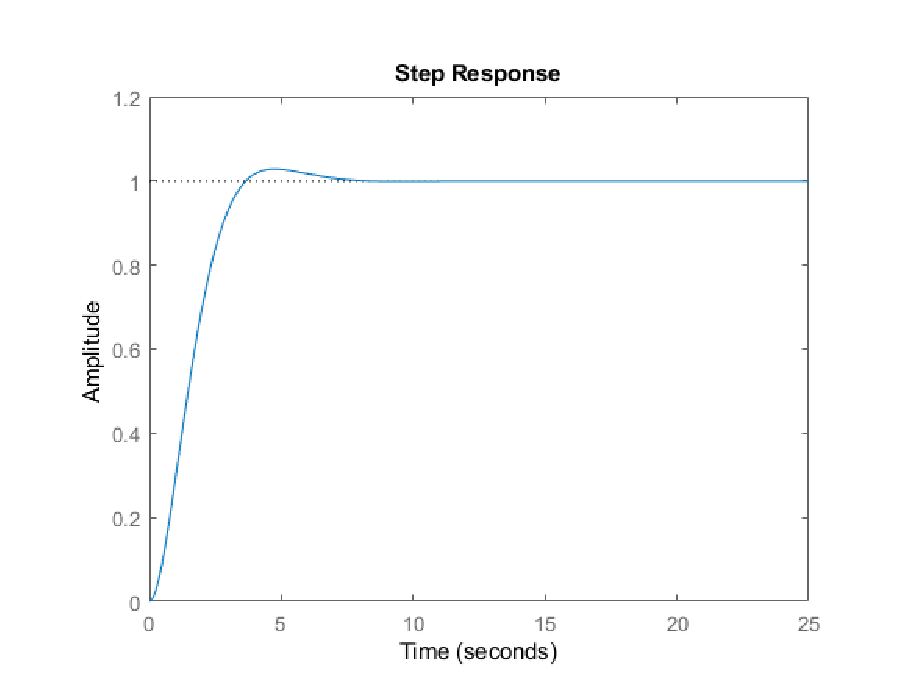
\includegraphics[width=\maxwidth{56.196688409433015em}]{figure_4.eps}
\end{center}
\begin{matlabcode}

%------------------------------------
% identifying the characteristics 
% of the transient response
stepinfo(G2)
\end{matlabcode}
\begin{matlaboutput}
ans = 
        RiseTime: 2.2884
    SettlingTime: 5.7426
     SettlingMin: 0.9049
     SettlingMax: 1.0284
       Overshoot: 2.8369
      Undershoot: 0
            Peak: 1.0284
        PeakTime: 4.7280

\end{matlaboutput}


\begin{matlabcode}
%------------------------------------
% defining the transfer function 

xi = 1;  

% define numerator and denominator
num = 1;
den = [1, 2*xi, 1];
G3 = tf(num, den)
\end{matlabcode}
\begin{matlaboutput}
G3 =
 
        1
  -------------
  s^2 + 2 s + 1
 
Continuous-time transfer function.
\end{matlaboutput}
\begin{matlabcode}

%------------------------------------
% plotting the step response

T = 25; % final time value

figure;
step(G3, T)
\end{matlabcode}
\begin{center}
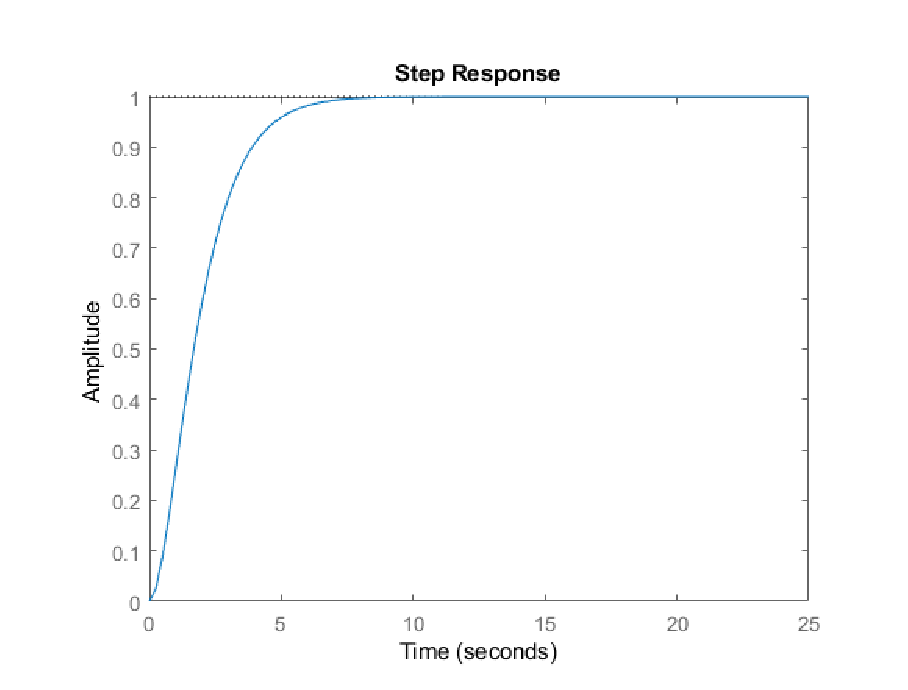
\includegraphics[width=\maxwidth{56.196688409433015em}]{figure_5.eps}
\end{center}
\begin{matlabcode}

%------------------------------------
% identifying the characteristics 
% of the transient response
stepinfo(G3)
\end{matlabcode}
\begin{matlaboutput}
ans = 
        RiseTime: 3.3579
    SettlingTime: 5.8339
     SettlingMin: 0.9000
     SettlingMax: 0.9994
       Overshoot: 0
      Undershoot: 0
            Peak: 0.9994
        PeakTime: 9.7900

\end{matlaboutput}


\begin{matlabcode}
%------------------------------------
% defining the transfer function 

xi = 2;  

% define numerator and denominator
num = 1;
den = [1, 2*xi, 1];
G4 = tf(num, den)
\end{matlabcode}
\begin{matlaboutput}
G4 =
 
        1
  -------------
  s^2 + 4 s + 1
 
Continuous-time transfer function.
\end{matlaboutput}
\begin{matlabcode}

%------------------------------------
% plotting the step response

T = 25; % final time value

figure;
step(G4, T)
\end{matlabcode}
\begin{center}
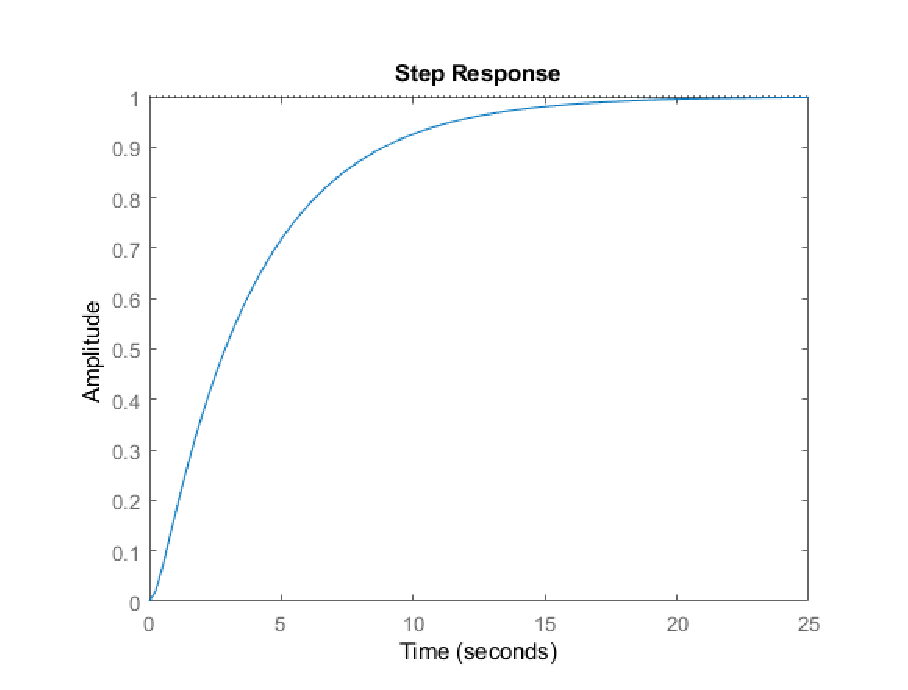
\includegraphics[width=\maxwidth{56.196688409433015em}]{figure_6.eps}
\end{center}
\begin{matlabcode}

%------------------------------------
% identifying the characteristics 
% of the transient response
stepinfo(G4)
\end{matlabcode}
\begin{matlaboutput}
ans = 
        RiseTime: 8.2308
    SettlingTime: 14.8789
     SettlingMin: 0.9017
     SettlingMax: 0.9993
       Overshoot: 0
      Undershoot: 0
            Peak: 0.9993
        PeakTime: 27.3269

\end{matlaboutput}


\matlabheading{\textit{Question 2 (4 marks)}}

\begin{par}
\begin{flushleft}
Consider the following open-loop unstable system.
\end{flushleft}
\end{par}

\begin{par}
$$Q(s)={{\frac{s+1}{s(s-1)(s+6)}}}$$
\end{par}

\begin{par}
\begin{flushleft}
A constant gain $k$ (controller) is used to stabilize this system. For different values of $k\in \lbrace 10,~20,~50,~100\rbrace$, plot the step response \textbf{(for 15 seconds)} of the closed-loop system and identify its characteristics using \texttt{\textbf{stepinfo}}.
\end{flushleft}
\end{par}

\begin{par}
\begin{flushleft}
\textless{}\textless{}fig\_lab02\_closedLoop.png\textgreater{}\textgreater{}
\end{flushleft}
\end{par}

\begin{matlabcode}
% There are 2 transfer functions that form an interconnected closed loop
% system. Here we define the first transfer function as "transferFunction1"
% and the 2nd "transferFucntion" for "k" will be defined per case. the transfer
% function for the interconnected system (considering the feedback will be
% then obtained based on "transferFunction1" and k (defined per case basis)

% Define the transfer function
gain = 1;
z = [-1];
p = [0, 1, -6];

transferFunction1 = zpk(z, p, gain) 
\end{matlabcode}
\begin{matlaboutput}
transferFunction1 =
 
      (s+1)
  -------------
  s (s-1) (s+6)
 
Continuous-time zero/pole/gain model.
\end{matlaboutput}


\begin{matlabcode}
%------------------------------------
% find the tranferFunction for the closed
% loop system 

k1 = 10;
connectedTransferFunction1 = feedback(transferFunction1, k1)
\end{matlabcode}
\begin{matlaboutput}
connectedTransferFunction1 =
 
               (s+1)
  --------------------------------
  (s+4.603) (s^2 + 0.397s + 2.173)
 
Continuous-time zero/pole/gain model.
\end{matlaboutput}
\begin{matlabcode}

%------------------------------------
% plot the step response 

T1 = 15; 
figure;
step(connectedTransferFunction1, T1)
\end{matlabcode}
\begin{center}
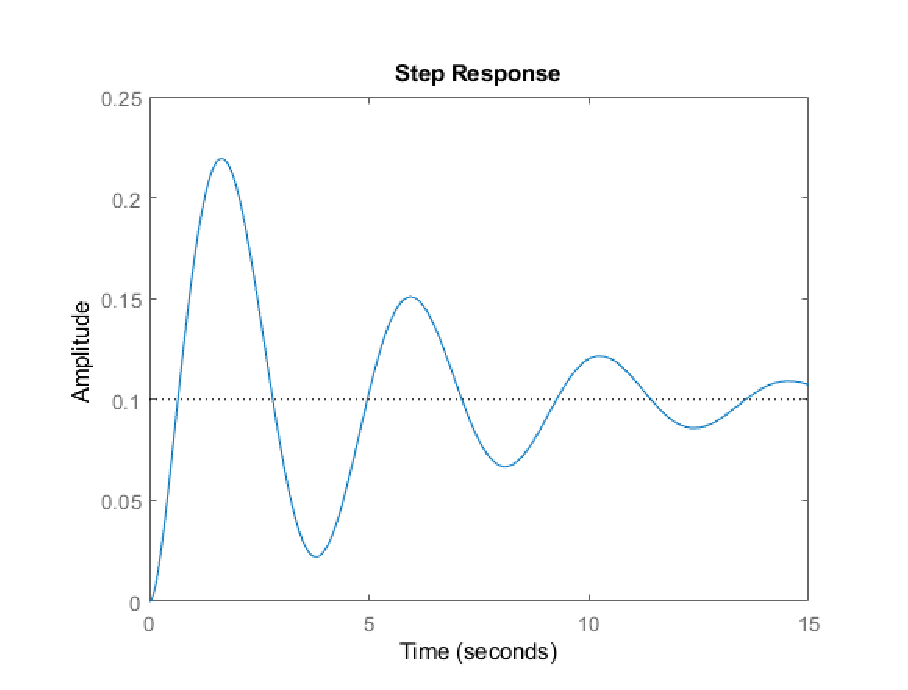
\includegraphics[width=\maxwidth{56.196688409433015em}]{figure_7.eps}
\end{center}
\begin{matlabcode}

%------------------------------------
% identifying the characteristics 
% of the response

stepinfo(connectedTransferFunction1)
\end{matlabcode}
\begin{matlaboutput}
ans = 
        RiseTime: 0.4424
    SettlingTime: 21.2506
     SettlingMin: 0.0221
     SettlingMax: 0.2194
       Overshoot: 119.3930
      Undershoot: 0
            Peak: 0.2194
        PeakTime: 1.6408

\end{matlaboutput}


\begin{matlabcode}
%------------------------------------
% find the tranferFunction for the closed
% loop system 

k2 = 20;
connectedTransferFunction2 = feedback(transferFunction1, k2)
\end{matlabcode}
\begin{matlaboutput}
connectedTransferFunction2 =
 
               (s+1)
  --------------------------------
  (s+2.579) (s^2 + 2.421s + 7.756)
 
Continuous-time zero/pole/gain model.
\end{matlaboutput}
\begin{matlabcode}

%------------------------------------
% plot the step response 

T1 = 15;
figure;
step(connectedTransferFunction2, T1)
\end{matlabcode}
\begin{center}
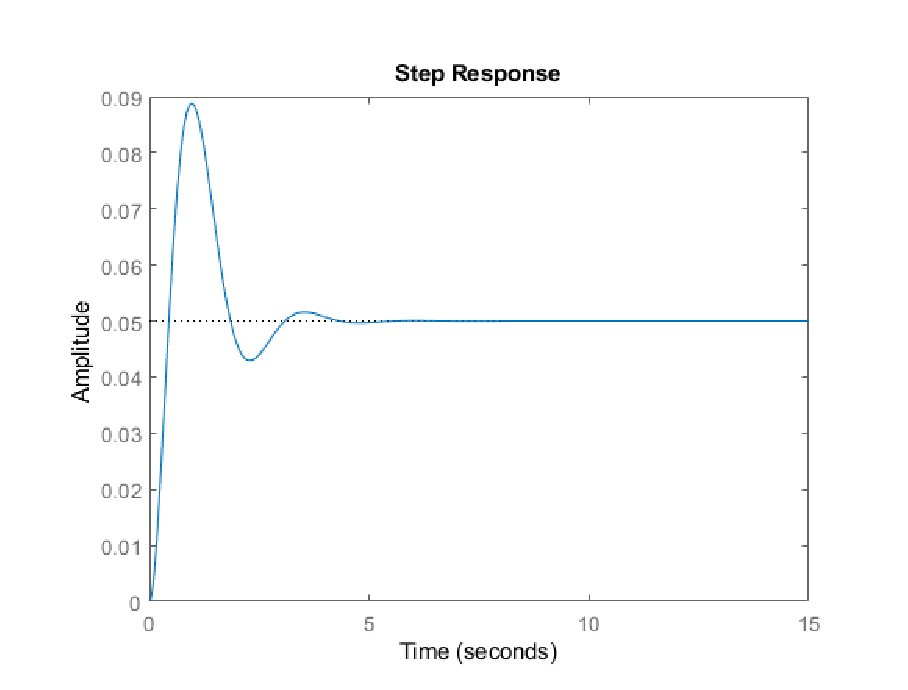
\includegraphics[width=\maxwidth{56.196688409433015em}]{figure_8.eps}
\end{center}
\begin{matlabcode}

%------------------------------------
% identifying the characteristics 
% of the response

stepinfo(connectedTransferFunction2)
\end{matlabcode}
\begin{matlaboutput}
ans = 
        RiseTime: 0.2989
    SettlingTime: 3.8974
     SettlingMin: 0.0430
     SettlingMax: 0.0889
       Overshoot: 77.7158
      Undershoot: 0
            Peak: 0.0889
        PeakTime: 0.9644

\end{matlaboutput}
\begin{matlabcode}


%------------------------------------
%-----------Conclusion---------------
% the system stabilizes quicker and 
% has a lower peak compared 
% to the previous case with smaller k
% (smaller Settling time and Peak in comparison with
% the previous case)
\end{matlabcode}


\begin{matlabcode}
%------------------------------------
% find the tranferFunction for the closed
% loop system 

k3 = 50;
connectedTransferFunction3 = feedback(transferFunction1, k3)
\end{matlabcode}
\begin{matlaboutput}
connectedTransferFunction3 =
 
               (s+1)
  --------------------------------
  (s+1.274) (s^2 + 3.726s + 39.25)
 
Continuous-time zero/pole/gain model.
\end{matlaboutput}
\begin{matlabcode}

%------------------------------------
% plot the step response 

T1 = 15;
figure;
step(connectedTransferFunction3, T1)
\end{matlabcode}
\begin{center}
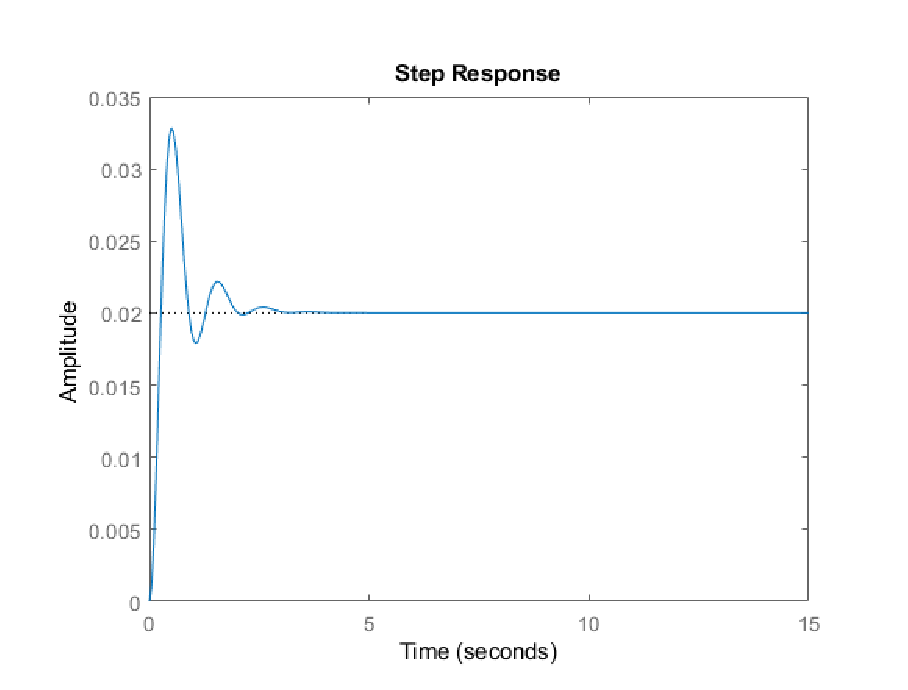
\includegraphics[width=\maxwidth{56.196688409433015em}]{figure_9.eps}
\end{center}
\begin{matlabcode}

%------------------------------------
% identifying the characteristics 
% of the response

stepinfo(connectedTransferFunction3)
\end{matlabcode}
\begin{matlaboutput}
ans = 
        RiseTime: 0.1767
    SettlingTime: 2.6377
     SettlingMin: 0.0179
     SettlingMax: 0.0329
       Overshoot: 64.3033
      Undershoot: 0
            Peak: 0.0329
        PeakTime: 0.5062

\end{matlaboutput}
\begin{matlabcode}


%------------------------------------
%-----------Conclusion---------------
% Again, the system stabilizes quicker and 
% has a lower peak compared 
% to the previous case with smaller k
% (smaller Settling time and Peak in comparison with
% the previous case)
\end{matlabcode}


\begin{matlabcode}
%------------------------------------
% find the tranferFunction for the closed
% loop system 

k4 = 100;
connectedTransferFunction4 = feedback(transferFunction1, k4)
\end{matlabcode}
\begin{matlaboutput}
connectedTransferFunction4 =
 
               (s+1)
  --------------------------------
  (s+1.115) (s^2 + 3.885s + 89.67)
 
Continuous-time zero/pole/gain model.
\end{matlaboutput}
\begin{matlabcode}

%------------------------------------
% plot the step response 
T1 = 15;
figure;
step(connectedTransferFunction4, T1)
\end{matlabcode}
\begin{center}
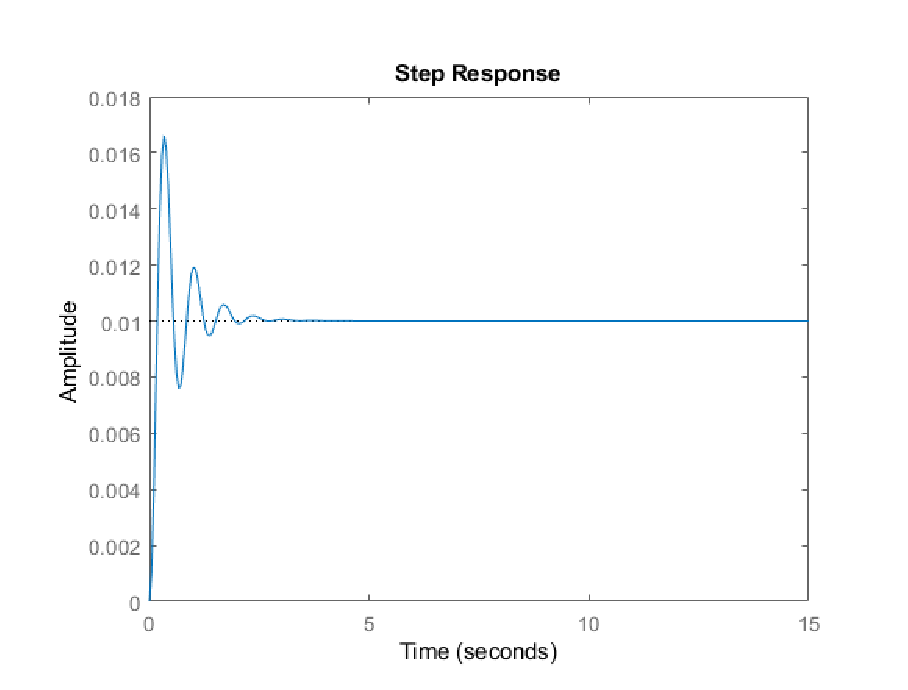
\includegraphics[width=\maxwidth{56.196688409433015em}]{figure_10.eps}
\end{center}
\begin{matlabcode}

%------------------------------------
% identifying the characteristics 
% of the response

stepinfo(connectedTransferFunction4)
\end{matlabcode}
\begin{matlaboutput}
ans = 
        RiseTime: 0.1190
    SettlingTime: 1.8674
     SettlingMin: 0.0076
     SettlingMax: 0.0166
       Overshoot: 66.0662
      Undershoot: 0
            Peak: 0.0166
        PeakTime: 0.3303

\end{matlaboutput}
\begin{matlabcode}


%------------------------------------
%-----------Conclusion---------------
% Again, the system stabilizes quicker and 
% has a lower peak compared 
% to the previous case with smaller k
% (smaller Settling time and Peak in comparison with
% the previous case)
\end{matlabcode}


\matlabheading{\textit{Question 3 (4 marks)}}

\begin{par}
\begin{flushleft}
Consider the closed-loop transfer function in Question 2.
\end{flushleft}
\end{par}

\begin{par}
$$T(s)={{\frac{kQ(s)}{1+kQ(s)}}}$$
\end{par}

\begin{par}
\begin{flushleft}
We would like to approximate this system to a second order system of the form:
\end{flushleft}
\end{par}

\begin{par}
$$G(s)={{\frac{{{\frac{k}{|p_3 |}(s-z_1 )}}}{(s-p_1 )(s-p_2 )}}}$$
\end{par}

\begin{enumerate}
\setlength{\itemsep}{-1ex}
   \item{\begin{flushleft} For $k=\lbrace 10,~20\rbrace$, find $p_1$, $p_2$ and $p_3$, where $p_1$ and $p_2$ are the dominant poles (i.e., poles with the smallest absolute real values) and $p_3$ is the ineffective pole(i.e., the pole with the largest absolute real value). \end{flushleft}}
   \item{\begin{flushleft} For $k=\lbrace 10,~20\rbrace$, plot the step response of the new second order system for \textbf{15 sec} and identify its characteristics using \texttt{\textbf{stepinfo}}. \end{flushleft}}
   \item{\begin{flushleft} For $k=\lbrace 10,~20\rbrace$, compare the step response with those obtained in Question 2. What do you observe? \end{flushleft}}
\end{enumerate}

\begin{par}
\begin{flushleft}
- 1)
\end{flushleft}
\end{par}

\begin{matlabcode}
% Find the pole(s) and zero(s) of the two transfer functions

% transfer functions with k = 10 
%-----------------------------------------------------------------------------------
connectedTransferFunction1 % Found in the previous question with k = 10 
\end{matlabcode}
\begin{matlaboutput}
connectedTransferFunction1 =
 
               (s+1)
  --------------------------------
  (s+4.603) (s^2 + 0.397s + 2.173)
 
Continuous-time zero/pole/gain model.
\end{matlaboutput}
\begin{matlabcode}
poles_k10 = pole(connectedTransferFunction1) % find the poles of the transfer function 
\end{matlabcode}
\begin{matlaboutput}
poles_k10 = 3x1 complex    
  -4.6030 + 0.0000i
  -0.1985 + 1.4605i
  -0.1985 - 1.4605i

\end{matlaboutput}
\begin{matlabcode}
zeros_k10 = zero(connectedTransferFunction1)
\end{matlabcode}
\begin{matlaboutput}
zeros_k10 = -1
\end{matlaboutput}
\begin{matlabcode}

% transfer functions with k = 20 
%-----------------------------------------------------------------------------------
connectedTransferFunction2 % Found in the previous question with k = 20
\end{matlabcode}
\begin{matlaboutput}
connectedTransferFunction2 =
 
               (s+1)
  --------------------------------
  (s+2.579) (s^2 + 2.421s + 7.756)
 
Continuous-time zero/pole/gain model.
\end{matlaboutput}
\begin{matlabcode}
poles_k20 = pole(connectedTransferFunction2) % find the poles of the transfer function 
\end{matlabcode}
\begin{matlaboutput}
poles_k20 = 3x1 complex    
  -1.2107 + 2.5081i
  -1.2107 - 2.5081i
  -2.5786 + 0.0000i

\end{matlaboutput}
\begin{matlabcode}
zeros_k20 = zero(connectedTransferFunction2)
\end{matlabcode}
\begin{matlaboutput}
zeros_k20 = -1
\end{matlaboutput}


\begin{par}
\begin{flushleft}
Transfer functions with dominant poles
\end{flushleft}
\end{par}

\begin{matlabcode}
% k = 10

% loop through the poles, find the complex 
% number with the max real value and store it in p3

for i = 1 : length(poles_k10)
    if abs(real(poles_k10(i))) == max(abs(real(poles_k10)))
        p3_k10 = poles_k10(i) % ineffective pole
    end
end
\end{matlabcode}
\begin{matlaboutput}
p3_k10 = -4.6030
\end{matlaboutput}
\begin{matlabcode}

% remove p3 from the poles
poles_k10(poles_k10 == p3_k10) = [];

% p1 and p2 will be the remaining poles
% dominant poles 
p1_k10 = poles_k10(1)
\end{matlabcode}
\begin{matlaboutput}
p1_k10 = -0.1985 + 1.4605i
\end{matlaboutput}
\begin{matlabcode}
p2_k10 = poles_k10(2)
\end{matlabcode}
\begin{matlaboutput}
p2_k10 = -0.1985 - 1.4605i
\end{matlaboutput}


\begin{matlabcode}
% k = 20

% loop through the poles, find the complex 
% number with the max real value and store it in p3

for i = 1 : length(poles_k20)
    if abs(real(poles_k20(i))) == max(abs(real(poles_k20)))
        p3_k20 = poles_k20(i) % ineffective pole
    end
end
\end{matlabcode}
\begin{matlaboutput}
p3_k20 = -2.5786
\end{matlaboutput}
\begin{matlabcode}

% remove p3 from the poles
poles_k20(poles_k20 == p3_k20) = [];

% p1 and p2 will be the remaining poles
% dominant poles 
p1_k20 = poles_k20(1)
\end{matlabcode}
\begin{matlaboutput}
p1_k20 = -1.2107 + 2.5081i
\end{matlaboutput}
\begin{matlabcode}
p2_k20 = poles_k20(2)
\end{matlabcode}
\begin{matlaboutput}
p2_k20 = -1.2107 - 2.5081i
\end{matlaboutput}


\begin{par}
\begin{flushleft}
- 2)
\end{flushleft}
\end{par}

\begin{matlabcode}
% k = 10

connectedTransferFunction1
\end{matlabcode}
\begin{matlaboutput}
connectedTransferFunction1 =
 
               (s+1)
  --------------------------------
  (s+4.603) (s^2 + 0.397s + 2.173)
 
Continuous-time zero/pole/gain model.
\end{matlaboutput}
\begin{matlabcode}

% define the approximated transfer function 
gain = 1;
z = [-1];
p = [p1_k10, p2_k10]; % don't include the ineffective pole p3_k10

tfApprox1 = zpk(z, p, gain)/abs(p3_k10)
\end{matlabcode}
\begin{matlaboutput}
tfApprox1 =
 
      0.21725 (s+1)
  ----------------------
  (s^2 + 0.397s + 2.173)
 
Continuous-time zero/pole/gain model.
\end{matlaboutput}
\begin{matlabcode}


%------------------------------------
% plot the step response 

T1 = 15;
figure;
step(tfApprox1, T1)
\end{matlabcode}
\begin{center}
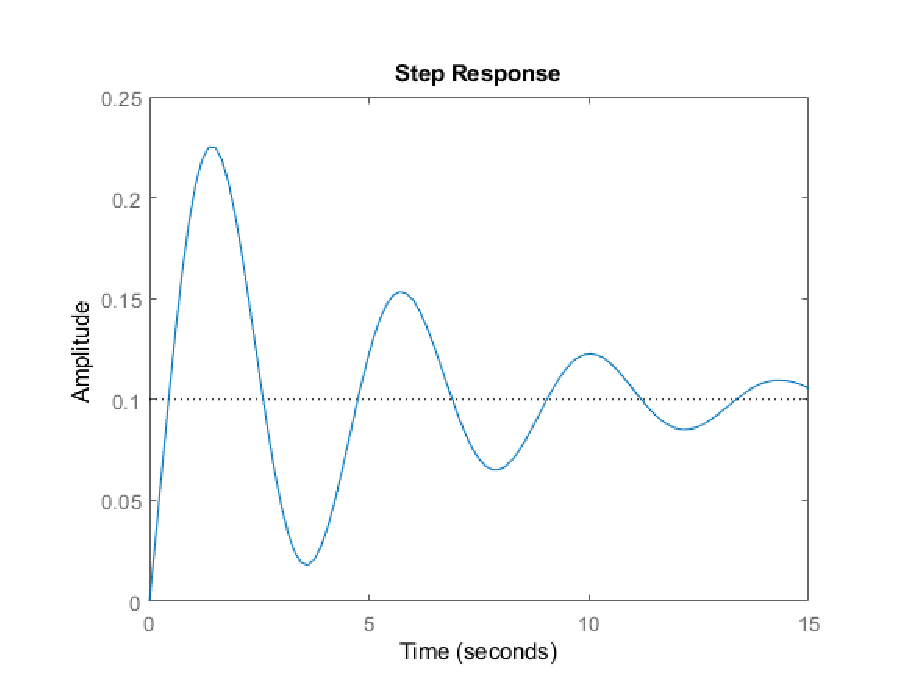
\includegraphics[width=\maxwidth{56.196688409433015em}]{figure_11.eps}
\end{center}
\begin{matlabcode}

%------------------------------------
% identifying the characteristics 
% of the response

stepinfo(tfApprox1)
\end{matlabcode}
\begin{matlaboutput}
ans = 
        RiseTime: 0.3487
    SettlingTime: 21.0226
     SettlingMin: 0.0182
     SettlingMax: 0.2250
       Overshoot: 124.9788
      Undershoot: 0
            Peak: 0.2250
        PeakTime: 1.4920

\end{matlaboutput}


\begin{matlabcode}
% k = 20

connectedTransferFunction2
\end{matlabcode}
\begin{matlaboutput}
connectedTransferFunction2 =
 
               (s+1)
  --------------------------------
  (s+2.579) (s^2 + 2.421s + 7.756)
 
Continuous-time zero/pole/gain model.
\end{matlaboutput}
\begin{matlabcode}

% define the approximated transfer function 
gain = 1;
z = [-1];
p = [p1_k20, p2_k20]; % don't include the ineffective pole p3_k20

tfApprox2 = zpk(z, p, gain)/abs(p3_k20)
\end{matlabcode}
\begin{matlaboutput}
tfApprox2 =
 
      0.38781 (s+1)
  ----------------------
  (s^2 + 2.421s + 7.756)
 
Continuous-time zero/pole/gain model.
\end{matlaboutput}
\begin{matlabcode}


%------------------------------------
% plot the step response 

T1 = 15;
figure;
step(tfApprox2, T1)
\end{matlabcode}
\begin{center}
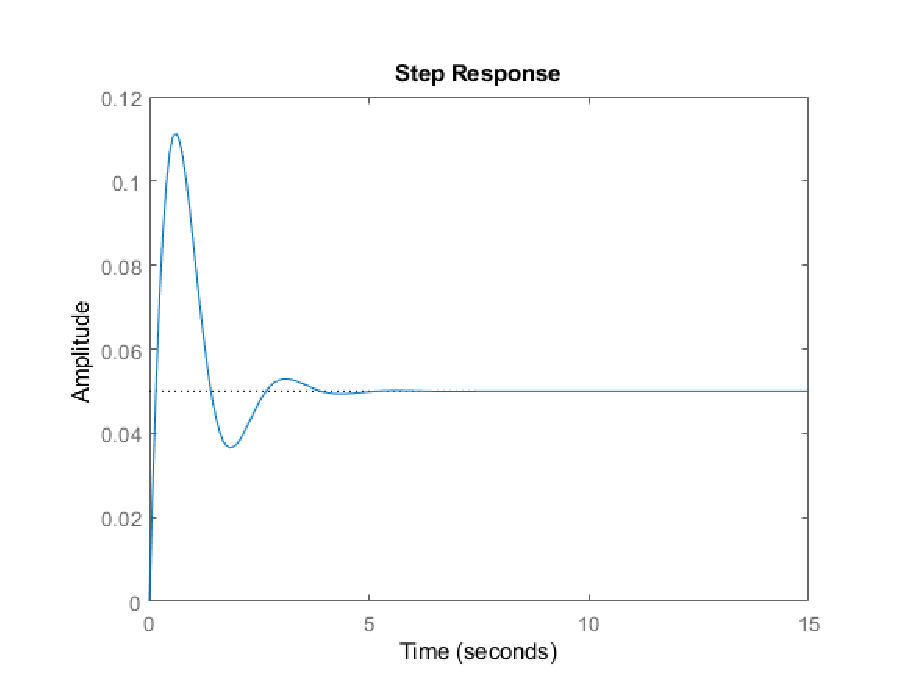
\includegraphics[width=\maxwidth{56.196688409433015em}]{figure_12.eps}
\end{center}
\begin{matlabcode}

%------------------------------------
% identifying the characteristics 
% of the response

stepinfo(tfApprox2)
\end{matlabcode}
\begin{matlaboutput}
ans = 
        RiseTime: 0.1163
    SettlingTime: 3.6016
     SettlingMin: 0.0365
     SettlingMax: 0.1113
       Overshoot: 122.6637
      Undershoot: 0
            Peak: 0.1113
        PeakTime: 0.6086

\end{matlaboutput}


\begin{par}
\begin{flushleft}
- 3)
\end{flushleft}
\end{par}

\begin{matlabcode}
% k = 10
%

% We can see by comparing the plots for the step response in q2 and the approximation in 
% q3 that the step response is very similar.  Going deeper and comparing the stepinfo
% (RiseTime, SettlingTime, Overshoot and ...), we can still see that values are very
% similar between the approximation and the step response in q2. 
% Even though the stepinfo values are a bit different for some properties 
% such as 

% OS: 119.3930 vs 124.9788
% Peaktime : 1.4920 vs 1.6408

% most are very close. We could therefore conclude that the approximation 
% we did in q3 for k=10 is valid and minimal info was lost and changed 
% between the approximation and the original step response 

\end{matlabcode}


\begin{matlabcode}
% k = 20
%

% We can see by comparing the plots for the step response in q2 and the
% approximation in q3 that the step responses look very similar. However,
% when we take a deeper look by comparing the stepinfo (RiseTime,
% SettlingTime, Overshoot and ...), we see some small but noticeable 
% differences. For example the following: 

% RiseTime : 0.2989 vs 1163
% Overshoot : 77.7158 vs 122.6637
% Peak :  0.1113 vs 0.0889 
% PeakTime : 0.9644 vs  0.6086

% The properties of the step response being more different than what we
% would consider acceptable for an approximation, we can conclude that the
% approximation done in q3 for k=20 is not very precise. 
\end{matlabcode}


\begin{matlabcode}
% As we saw, the approximation for k=10 was more successful than the
% approximation for k=20. 

% The main reason I find for this difference between the 2 cases are the
% poles. As we know we can perform dominant pole approximation if
% |Re(pole)| > 0.1*|Re(other pole)| or |Re(pole)| > 0.2*|Re(other pole)|.
% If we take a look at the poles, for "connectedTransferFunction1" (k=10),
% we have the following poles:

% -4.6030
% -0.1985 + 1.4605 i 
% -0.1985 - 1.4605 i
% and we see that 
% |-4.6030| > 10 * |-0.1985|
% So the dominant pole approximation is valid

% for "connectedTransferFunction2" (k=20), we have the following poles: 

% -2.5786  
% -1.2107 + 2.5081 i
% -1.2107 - 2.5081 i
% and we see that 
% |-2.5786| !> 10 * |-1.2107| 
% So the dominant pole approximation shouldn't be considered

% This is the main reason one approximation is more accurate than the other
% in our case


\end{matlabcode}

\end{document}
